\section{A Fitted Lens Reports the Language of Its Fitting Corpus}
\label{sec:beyond-token}
\label{sec:readout-analyses}
\label{subsec:cross-lens}

A fitted lens maps an intermediate hidden state into the space consumed
by the LM head. The resulting tokens are often interpreted as evidence
about the information represented at that layer, including the language
in which the model is operating. For example,
\citet{gurnee2026workspace} obtain English tokens from intermediate
states for a Chinese prompt and interpret them as evidence that the
intermediate computation occurs in English.

Because this map is learned from a corpus, its token readings can reflect
both the hidden state and the fitting corpus, and a token ranking alone
cannot distinguish these sources. We call this dependence corpus
conditionality. The fitting corpus affects the lens through the learned
map \(\rstate=T_\ell(h_\ell)\) (\S\ref{sec:method}), so our results apply
only to fitted lenses. Studies of latent language that decode states
directly through the unembedding use no fitting corpus
\citep{wendler2024llamas,schut2025english} and are therefore not subject
to this dependence. Appendix~\ref{app:extended-related-work} discusses a
separate confound in token readings that affects those studies.

\subsection{Design}
\label{subsec:cross-lens-design}
We test corpus conditionality by holding an intermediate hidden state
\(h_\ell\) fixed and varying only the corpus used to fit the lens. The
two fitted maps can produce different decoded states from the same
state, and hence different token readings, so any difference between
the readings is attributable to the fitting corpus. To
test whether different tokens reflect different readout structure, SRP
decomposes both selected token scores in a single basis learned only
from the model weights. Translation pairs, language labels, and fitting
corpora do not enter this basis, which provides a reference independent
of the fitting corpus.

Using the reference implementation, we fit two Jacobian lenses
\citep{gurnee2026workspace} on Qwen3.5-9B. The first uses 100 English C4
prompts, and the second uses 100 Chinese C4 prompts. We hold seeds,
layers, and all other procedures fixed. We apply both lenses to the same
frozen states from 80 evaluation prompts spanning seven task families.
We also evaluate 12 controls---six digit prompts and six proper noun
prompts---whose expected outputs are language invariant.

We evaluate layers 21, 24, 26, and 29, where the two lenses can
produce different token readings. At each layer, we decompose the score
assigned to the token reported by each lens and record the feature with
the largest contribution in absolute value
(\S\ref{sec:method-comparing-accounts}). We count a prompt as agreement
when the same feature dominates under both lenses in at least two of the
four layers. Requiring two of the four layers keeps a match at one
layer alone from counting as agreement. We use two null comparisons to
estimate chance agreement under this rule. One evaluates an unrelated token under the same lens,
and the other shuffles prompts before pairing the two lenses.
Appendix~\ref{app:cross-lens} provides the full protocol, token and
feature agreement rates for each family, and results for each prompt.

\begin{figure}[t]
    \centering
    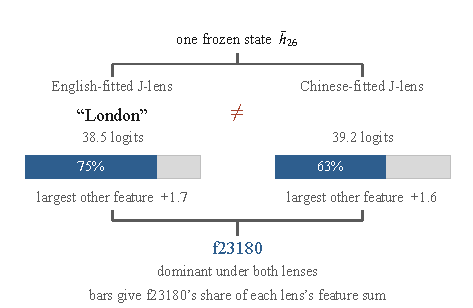
\includegraphics[width=\columnwidth]{figures/cross_lens/cross_lens_shared_feature.pdf}
    \caption{\textbf{Two lenses, two surface languages, one readout
    feature.} The figure shows a Chinese factual recall prompt, which
    translates as ``The capital of China is Beijing. The capital of the
    UK is \ldots''. For the same frozen Qwen3.5-9B state at layer 26, the
    Jacobian lens fitted on English reports \texttt{London}, whereas the
    lens fitted on Chinese reports
    \begin{CJK*}{UTF8}{gbsn}伦敦\end{CJK*} (``London''). Below each token
    is its logit under the corresponding lens. The bar shows the share
    of the lens's feature sum attributable to the shared readout feature
    f23180, which dominates both scores. The feature sum is the signed
    sum of the feature contributions and excludes the offset and the
    residual.}
    \label{fig:cross-lens-butterfly}
\end{figure}

\subsection{Different Tokens Share a Dominant Feature}
\label{subsec:cross-lens-token-conflict}
\label{subsec:cross-lens-feature-invariance}
Across layers 21, 24, 26, and 29, the two lenses report tokens in
different scripts on 39 of 80 prompts, while their outputs converge at the
final layer. On factual recall prompts, the lenses report different
scripts on 9 of 10 (\Cref{fig:cross-lens-butterfly}). On the antonym
prompt from \citet{gurnee2026workspace}, the lens fitted on English reports
\texttt{large} at layers 24 and 26 and \texttt{big} at layer 29. The
lens fitted on Chinese instead reports
\begin{CJK*}{UTF8}{gbsn}大的\end{CJK*} (``large'' or ``the large one'')
at layers 24 and 26 and
\begin{CJK*}{UTF8}{gbsn}大\end{CJK*} (``large'' or ``big'') at layer
29. Interpreting either lens alone would therefore yield opposing
conclusions about the model's intermediate language.

The same SRP feature dominates under both lenses on 77 of 80 prompts
(96\%, 95\% CI [0.90, 0.99]). In
\Cref{fig:cross-lens-butterfly}, f23180 accounts for 75\% of the feature
sum for the lens fitted on English and 63\% for the lens fitted on
Chinese. Every other feature contributes at most \(+1.7\) logits.
Neither null comparison produces a match, with 0/159 for unrelated
tokens and 0/240 after shuffling prompts.
The dominant feature agrees under both lenses on 5/6 digit controls and
5/6 proper noun controls.

\begin{figure}[t]
    \centering
    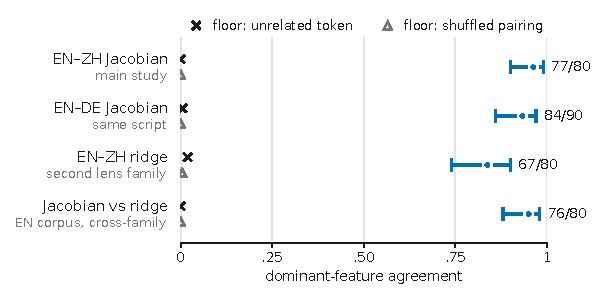
\includegraphics[width=\columnwidth]{figures/cross_lens/cross_lens_extension_matrix.pdf}
    \caption{\textbf{Feature agreement across language pairs and lens
    constructions.} A prompt counts as agreement when the same
    feature dominates under both lenses in at least two of layers 21,
    24, 26, and 29. Points show agreement rates, intervals show 95\%
    binomial CIs, and counts appear at the right. Two baseline markers per
    setting show the matched null rates. All eight are at most 3/159
    (1.9\%). Appendix~\ref{app:cross-lens} provides tables for each
    family and construction details.}
    \label{fig:cross-lens-extension}
\end{figure}

\subsection{The Pattern Persists Across Languages, Lens Constructions, and Corpus Sizes}
\label{subsec:cross-lens-extensions}
We extend the corpus conditionality analysis across a second lens
construction, a language pair that shares a script, and larger fitting
corpora. In each extension we test whether the token readings change while
the same readout feature remains dominant.
\Cref{fig:cross-lens-extension} reports the agreement rates and matched
null comparisons.

\paragraph{Lens construction.}
We fit ridge translators related to the tuned lens
\citep{belrose2023tuned} on the same English and Chinese corpora of 100
prompts. On 9 of 10 EN\(\to\)ZH translation
prompts, the translator fitted on English reads Latin tokens and the
translator fitted on Chinese reads CJK tokens. The same feature remains
dominant under both translators on 67/80 prompts (CI [0.74, 0.90]),
compared with 3/159 and 1/240 matches under the two null comparisons.
We then hold the English fitting corpus fixed to isolate the effect of
lens construction. The Jacobian lens and ridge translator agree on the
dominant feature for 76/80 prompts, and both null comparisons yield zero
matches.

\paragraph{Shared script.}
We next test English and German, which share the Latin script, and
exclude cognates from the evaluation set. The Jacobian lenses fitted on
English and German report different top-1 tokens on 73/90 prompts. The
same feature remains dominant on 84/90 prompts, compared with 1/204 and
0/270 matches under the two null comparisons. The dissociation therefore
does not depend on the distinct scripts used in the English--Chinese
comparison.

\paragraph{Corpus size.}
Finally, we triple each fitting corpus from 100 to 300 prompts to test
whether the original corpus size accounts for the disagreement. Feature
agreement remains 77/80 for English--Chinese and increases from 84/90
to 85/90 for English--German. Token disagreement moves in opposite
directions, falling from 39/80 to 33/80 for English--Chinese and rising
from 73/90 to 76/90 for English--German. Estimation noise that decreases
with additional fitting data would predict a decrease for both language
pairs. Across the two fitting scales, eleven English--Chinese prompts
change their reported language, and none changes its dominant feature.

On Qwen3.5-9B, the token readings vary with the language and size of
the fitting corpus, while the dominant readout feature remains stable
across these changes and across two lens constructions.
